
\documentclass[12pt]{article}

% Layout.
\usepackage[top=1in, bottom=0.75in, left=1in, right=1in, headheight=1in, headsep=6pt]{geometry}

% Fonts.
\usepackage{mathptmx}
\usepackage[scaled=0.86]{helvet}
\renewcommand{\emph}[1]{\textsf{\textbf{#1}}}

% TiKZ.
\usepackage{tikz, pgfplots}
\usetikzlibrary{calc}
\pgfplotsset{compat = newest}
 
\pgfplotsset{my style/.append style={axis x line=middle, axis y line=
middle, xlabel={$x$}, ylabel={$y$}, axis equal }}

% Misc packages.
\usepackage{amsmath,amssymb,latexsym}
\usepackage{graphicx}
\usepackage{array}
\usepackage{xcolor}
\usepackage{multicol}

% Commands to set various header/footer components.
\makeatletter
\def\doctitle#1{\gdef\@doctitle{#1}}
\doctitle{Use {\tt\textbackslash doctitle\{MY LABEL\}}.}
\def\docdate#1{\gdef\@docdate{#1}}
\docdate{Use {\tt\textbackslash docdate\{MY DATE\}}.}
\def\doccourse#1{\gdef\@doccourse{#1}}
\let\@doccourse\@empty
\def\docscoring#1{\gdef\@docscoring{#1}}
\let\@docscoring\@empty
\def\docversion#1{\gdef\@docversion{#1}}
\let\@docversion\@empty
\makeatother

% Headers and footers layout.
\makeatletter
\usepackage{fancyhdr}
\pagestyle{fancy}
\fancyhf{} % Clears all headers/footers.
\lhead{\baselineskip 30pt
%\emph{\@doctitle\hfill\@docdate}
\emph{\@docdate\hfill\@doctitle}
\ifnum \value{page} > 1\relax\else\\
\emph{Name: \rule{3.5in}{1pt}\hfill \@docscoring}\fi}
\rfoot{\emph{\@docversion}}
\lfoot{\emph{\@doccourse}}
\cfoot{\emph{\thepage}}
\renewcommand{\headrulewidth}{0pt}%
\makeatother

% Paragraph spacing
\parindent 0pt
\parskip 6pt plus 1pt

% A problem is a section-like command. Use \problem{5} to
% start a problem worth 5 points.
\newcounter{probcount}
\newcounter{subprobcount}
\setcounter{probcount}{0}
\newcommand{\problem}[1]{%
\par
\addvspace{4pt}%
\setcounter{subprobcount}{0}%
\stepcounter{probcount}%
\makebox[0pt][r]{\emph{\arabic{probcount}.}\hskip1ex}\emph{[#1 points]}\hskip1ex}
\newcommand{\thesubproblem}{\emph{\alph{subprobcount}.}}

% Subproblems are an enumerate-like environment with a consistent
% numbering scheme. 
% Use \begin{subproblems}\item...\item...\end{subproblems}
\newenvironment{subproblems}{%
\begin{enumerate}%
\setcounter{enumi}{\value{subprobcount}}%
\renewcommand{\theenumi}{\emph{\alph{enumi}}}}%
{\setcounter{subprobcount}{\value{enumi}}\end{enumerate}}

% Blanks for answers in normal and math mode.
\newcommand{\blank}[1]{\rule{#1}{0.75pt}}
\newcommand{\mblank}[1]{\underline{\hspace{#1}}}
\def\emptybox(#1,#2){\framebox{\parbox[c][#2]{#1}{\rule{0pt}{0pt}}}}

% Misc.
\renewcommand{\d}{\displaystyle}
\newcommand{\ds}{\displaystyle}
\def\bc{\begin{center}}
\def\ec{\end{center}}
\def\be{\begin{enumerate}}
\def\ee{\end{enumerate}}


\doctitle{Math 251: Quiz 2}
\docdate{September 8, 2023}
\doccourse{UAF Calculus I}
\docversion{v-1, async}
\docscoring{\blank{0.8in} / 25}
\begin{document}
%\textbf{Please circle your instructor's name:} \hfill Leah Berman  \hfill   Jill Faudree\\

\newcommand{\ans}{\blank{0.8in}}

There are 25 points possible on this quiz. {\it You should be able to complete it without using your notes or textbook -- this is practice for your exams!} If you needed to look something up, you might want to come talk to me about questions you might have.  {\bf Show all work for full credit} and use some words or sentences to help communicate your answers.

\problem{11} The point $P = (2,1)$ is a point on the graph of $f(x)=\frac{x}{3 - x} - 1$.
\begin{subproblems}
\item Find the slope of the secant line passing through $P$ and the point $Q = (0,f(0))$. Show some work.
\vfill
\hfill Slope = \ans

\item Find the slope of the secant line passing through $P$ and the point $R = (1,f(1))$. Show some work.

\vfill
\hfill Slope = \ans

\item The table below lists the slope of the secant line passing through the point $P$ and the point $S = (x, f(x))$ for several values of $x.$ The value $m_{\text{sec}}$ is the slope of the secant line.\\

\begin{tabular}{l || c|c|c||c|c|c}
$x$& 1.9 & 1.99 & 1.999& 2.001&2.01 &2.1 \\
\hline
$f(x)$&0.727273 & 0.970297 & 0.997003 & 1.003 &1.0303  &1.33333  \\
\hline \hline
$m_{\text{sec}}$&2.72727 &2.97030  & 2.99700 & 3.00300 &3.03030  & 3.33333 \\
\end{tabular}

\vskip 0.25cm
Use the information in the table to estimate the slope of the tangent line to $f(x)$ at the point $P=(2,1).$
%\vfill

\hfill Tangent line slope = \ans
\item Use the slope from part (c) above to write an equation of the tangent line at point $P = (2,1).$ You may write the equation of the line in whatever form you choose.

\vfill
\hfill Tangent line equation: \ans\ans\ans\ans


\item \quad 

\begin{minipage}{.4 \textwidth}
To the right is a sketch of part of the graph of \[f(x)=\displaystyle{\frac{x}{3 - x} - 1 }.\] \\
Sketch and label the \emph{tangent} line to the graph at the point $P=(2,1).$\\
Sketch and label the \emph{secant} line between $P=(2,1)$ and $Q=(0,f(0)).$
\end{minipage}
\hspace{1.5cm}
\begin{minipage}{.5\textwidth}
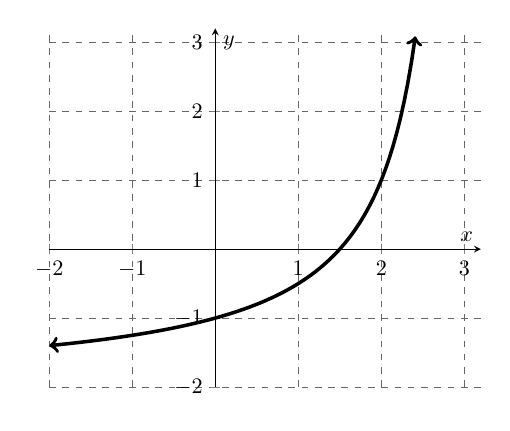
\begin{tikzpicture}[scale = .8]
 \begin{axis}[
    xmin = -2, xmax = 3.2,
    ymin = -2, ymax = 3.2, xtick={-2,-1,0,1,2, 3}, ytick={-2,-1,0,1,2,3},
    grid=both, grid style={ thin, black!60, dashed},axis x line=middle, axis y line=
middle, xlabel={$x$}, ylabel={$y$}]
    \addplot[ultra thick, <-> ,samples=100,
        domain = -2:2.41,
    ] {x/(3 - x) - 1};
    %\addplot[thick,->] coordinates {(-1,0) (6,0)};
    %%-x-\frac{6}{x+2}+7
    \end{axis}
\end{tikzpicture}
\end{minipage}
%

\end{subproblems}
\newpage


\problem{2} Use the right triangle below, with side lengths 8, 3 and missing value $c$, to evaluate the expressions. Give your answers as exact numbers. \\

\vspace{.1in}

\begin{multicols}{2}
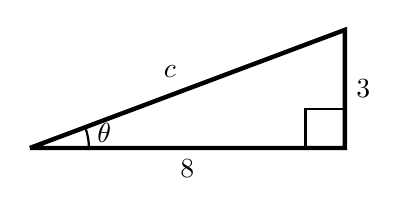
\begin{tikzpicture}[scale=0.5]
\draw[ultra thick] (0,0) -- node[below]{8} (8,0) -- node[right]{3} (8,3) -- node[above left]{$c$} (0,0);
%\node at (6,-1){12}; 
%\node at (13,2.5){5}; \node at (6,4){13};
%\draw [ultra thick,domain=0:25] plot ({3*cos(\x)}, {3*sin(\x)});

%\node at (4,.9){$\theta$};
\draw[thick] (8,0) rectangle (8-1, 1);
%\draw (11,0) -- (11,1) -- (12,1);
\draw[thick]  ($(0,0) + (0:1.5)$) arc (0:atan(3/8):1.5) node[ right, pos = .7]{$\theta$};
\end{tikzpicture}
\begin{subproblems}
\item $\displaystyle \tan (\theta) =$

\hspace{2cm}
\item $\displaystyle \sec (\theta) =$
\end{subproblems}
\end{multicols}
%\vspace{.5in}

\problem{8} Evaluate the expressions below. Assume all angles are measured in radians.\\


\begin{subproblems}
\begin{multicols}{2}
	\item $\displaystyle \sin (4 \pi /3)= $
	\item $\displaystyle \cos( \pi /2)=$
\end{multicols}
\vspace{1in}	
\begin{multicols}{2}
	\item $\displaystyle \tan ( 7 \pi /6)= $
	\item $\displaystyle \sin (- \pi /4) =$
\end{multicols}
\vspace{1in}
\end{subproblems}

\problem{4} An athlete is running along a straight path. The position of the athlete is given by $d(t)=\frac{1}{2} t^2+t,$ where $t$ is time measured in seconds and $d$ is distance measured in meters. Find the average velocity of the athlete between $t=2$ and $t=5.$ Include units with your answer.
\vfill
	
\end{document}